\ylDisplay{Takistid} % Ülesande nimi
{Aigar Vaigu} % Autor
{lõppvoor} % Voor
{2005} % Aasta
{G 4} % Ülesande nr.
{4} % Raskustase
{
% Teema: Elektriahelad
\ifStatement
Mitu korda muutub joonisel kujutatud ahelas takistil $A$ eralduv võimsus, kui vahetada alalispingeallika polaarsus? Kõik takistid on võrdse takistusega.

\begin{center}
	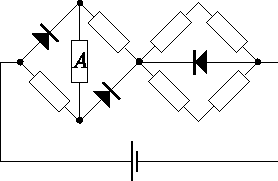
\includegraphics[width=0.6\linewidth]{2005-v3g-04-yl}
\end{center}
\fi


\ifHint
Teades, et päripidise voolu korral võib dioodi klemmid lugeda lühistatuks ning vastuvoolu korral isoleerituks, võib koostada esialgse skeemi asemel mõlema polaarsuse korral dioodideta ekvivalentsed skeemid.
\fi


\ifSolution
Paneme tähele, et pinge absoluutväärtus ahela otstele $U$ ei muutu. Arvestades, et päripidise voolu korral võib dioodi klemmid lugeda lühistatuks ning vastuvoolu korral isoleerituks, saame kummagi polaarsuse jaoks koostada algse ahela (joonis \ref{2005-v3g-04:fig1}) asemele ekvivalentsed ahelad (joonised \ref{2005-v3g-04:fig2} ja \ref{2005-v3g-04:fig3}).

\begin{figure}[h]
	\centering
	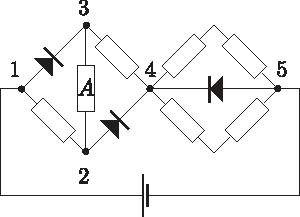
\includegraphics[width=0.6\linewidth]{2005-v3g-04-lah1}
	\caption{Esialgne skeem}
	\label{2005-v3g-04:fig1}
\end{figure}
\begin{figure}[h]
	\centering
	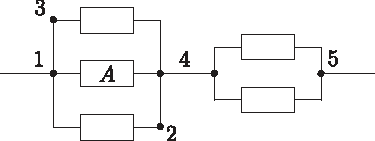
\includegraphics[width=0.6\linewidth]{2005-v3g-04-lah2}
	\caption{Ekvivalentne skeem ühe polaarsuse puhul}
	\label{2005-v3g-04:fig2}
\end{figure}
\begin{figure}[h]
	\centering
	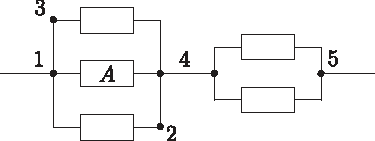
\includegraphics[width=0.6\linewidth]{2005-v3g-04-lah2}
	\caption{ Ekvivalentne skeem teise polaarsuse puhul}
	\label{2005-v3g-04:fig3}
\end{figure}

Leiame takistil $A$ eralduva võimsuse päripinge puhul. 

Takistil $A$ eralduv võimsus on $P_1 = I_1^2R$, kus
\[
I_1 = \frac{I}{3} = \frac{1}{3} \frac{U}{r_1}
\]
on vaadeldavat takistit läbiva voolu tugevus ning
\[
r_1 = \frac{R}{3} + R = \frac{4}{3} R
\]
on kogu ahela takistus. Seega
\[
P_1=\frac{R}{9} \frac{U^{2}}{r_{1}^{2}}=\frac{U^{2}}{R} \frac{1}{9} \frac{9}{16}=\frac{1}{16} \frac{U^{2}}{R}.
\]

Nüüd määrame takistil $A$ eralduva võimsuse vastupidise polaarsusega. 

Takistit $A$ läbib vool $I_2 = U/3R$. Seega võimsus on
\[
P_{2}=\left(\frac{U}{3 R}\right)^{2} R=\frac{1}{9} \frac{U^{2}}{R}.
\]
Võimsuste suhe
\[
\frac{P_1}{P_2} = \frac{9}{16},
\]
seega polaarsuse muutmisel muutub takistil $A$ eralduv võimsus $9/16$ korda.
\fi
}